\section{eo\-Vl\-Add\-Mutation$<$ EOT $>$ Class Template Reference}
\label{classeo_vl_add_mutation}\index{eoVlAddMutation@{eoVlAddMutation}}
Addition of a gene Is inserted at a random position - so can be applied to both order-dependent and order-independent.  


{\tt \#include $<$eo\-Variable\-Length\-Mutation.h$>$}

Inheritance diagram for eo\-Vl\-Add\-Mutation$<$ EOT $>$::\begin{figure}[H]
\begin{center}
\leavevmode
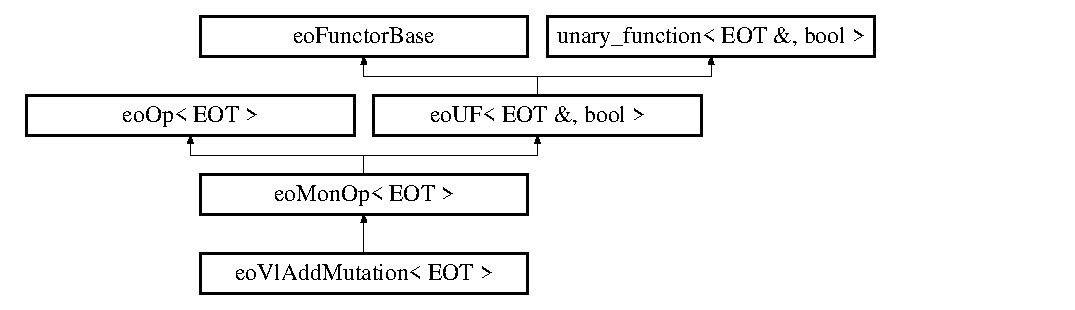
\includegraphics[height=3.71476cm]{classeo_vl_add_mutation}
\end{center}
\end{figure}
\subsection*{Public Types}
\begin{CompactItemize}
\item 
typedef EOT::Atom\-Type {\bf Atom\-Type}\label{classeo_vl_add_mutation_w0}

\end{CompactItemize}
\subsection*{Public Member Functions}
\begin{CompactItemize}
\item 
{\bf eo\-Vl\-Add\-Mutation} (unsigned \_\-n\-Max, {\bf eo\-Init}$<$ Atom\-Type $>$ \&\_\-atom\-Init)
\begin{CompactList}\small\item\em default ctor \item\end{CompactList}\item 
bool {\bf operator()} ({\bf EOT} \&\_\-eo)\label{classeo_vl_add_mutation_a1}

\begin{CompactList}\small\item\em operator: actually adds an Atom \item\end{CompactList}\item 
virtual std::string {\bf class\-Name} () const \label{classeo_vl_add_mutation_a2}

\begin{CompactList}\small\item\em inherited class\-Name \item\end{CompactList}\end{CompactItemize}
\subsection*{Private Attributes}
\begin{CompactItemize}
\item 
unsigned {\bf n\-Max}\label{classeo_vl_add_mutation_r0}

\item 
{\bf eo\-Init}$<$ Atom\-Type $>$ \& {\bf atom\-Init}\label{classeo_vl_add_mutation_r1}

\end{CompactItemize}


\subsection{Detailed Description}
\subsubsection*{template$<$class EOT$>$ class eo\-Vl\-Add\-Mutation$<$ EOT $>$}

Addition of a gene Is inserted at a random position - so can be applied to both order-dependent and order-independent. 



Definition at line 48 of file eo\-Variable\-Length\-Mutation.h.

\subsection{Constructor \& Destructor Documentation}
\index{eoVlAddMutation@{eo\-Vl\-Add\-Mutation}!eoVlAddMutation@{eoVlAddMutation}}
\index{eoVlAddMutation@{eoVlAddMutation}!eoVlAddMutation@{eo\-Vl\-Add\-Mutation}}
\subsubsection{\setlength{\rightskip}{0pt plus 5cm}template$<$class EOT$>$ {\bf eo\-Vl\-Add\-Mutation}$<$ {\bf EOT} $>$::{\bf eo\-Vl\-Add\-Mutation} (unsigned {\em \_\-n\-Max}, {\bf eo\-Init}$<$ Atom\-Type $>$ \& {\em \_\-atom\-Init})\hspace{0.3cm}{\tt  [inline]}}\label{classeo_vl_add_mutation_a0}


default ctor 

\begin{Desc}
\item[Parameters:]
\begin{description}
\item[{\em n\-Max}]max number of atoms \item[{\em \_\-atom\-Init}]an Atom initializer \end{description}
\end{Desc}


Definition at line 59 of file eo\-Variable\-Length\-Mutation.h.

The documentation for this class was generated from the following file:\begin{CompactItemize}
\item 
eo\-Variable\-Length\-Mutation.h\end{CompactItemize}
